The training part contains the 6 following functionalities:

\begin{itemize}
\item \mintinline{python}{romc.solve_problems(n1, use_bo=False, optimizer_args=None, seed=None)}
\item \mintinline{python}{romc.estimate_regions(eps_filter,}
  
      \mintinline{python}{                      use_surrogate=None, region_args=None,}
  
      \mintinline{python}{                      fit_models=False, fit_models_args=None,}
  
      \mintinline{python}{                      eps_region=None, eps_cutoff=None)}
      
    \item \mintinline{python}{romc.fit_posterior(n1, eps_filter, use_bo=False, optimizer_args=None,}
  
          \mintinline{python}{                   seed=None, use_surrogate=None, region_args=None,}
  
          \mintinline{python}{                   fit_models=False, fit_models_args=None,}
  
          \mintinline{python}{                   eps_region=None, eps_cutoff=None)}

\item \mintinline{python}{romc.distance_hist(savefig=False, **kwargs)}
\item \mintinline{python}{romc.visualize_region(i, savefig=False)}
\item \mintinline{python}{romc.compute_eps(quantile)}
\end{itemize}


\subsubsection*{Function (i): Define and solve the optimisation problems}

\pinline{romc.solve_problems(n1, use_bo=False, optimizer_args=None, seed=None)}
\vspace{5mm}

\noindent
This routine is responsible for (a) drawing the nuisance variables,
(b) define the optimisation problems and (c) solve them using either a
gradient-based optimiser or Bayesian optimisation. The aforementioned
tasks are done in a sequential fashion, as show in
figure~\ref{fig:elfi-model}. The defininition of the optimisation
problems is performed by drawing $n_1$ integer numbers from a discrete
uniform distribution $u_i \sim \mathcal{U}\{1, 2^{32}-1\}$. Each
integer $u_i$ is the seed used in ELFI's random simulator. Hence from
an algorithmic point-of-view drawing the state of all random
variables $\vb_i$ as described in the previous chapter, traces back to
just setting the seed that initialises the state of the pseudo-random
generator, before asking a sample from the simulator.

Finally, passing an integer number as the argument \pinline{seed}
absorbs all the randomness of the optimistation part (e.g.\ drawing
initial points for the optimisation procedure), making the whole
process reproducible.

Setting the argument \pinline{use_bo=True}, chooses the Bayesian
Optimisation scheme for obtaining $\theta_i^*$. In this case the
function $g_i(\thetab) = d(M_d(\thetab,\vb=\vb_i))$ which by default
is evaluated using the simulator, is replaced by a Gaussian Proccess
surrogate model $\hat{d}$, which is used in all next steps.

\subsubsection*{Function (ii): Construct bounding boxes and fit local surrogate models}

\mintinline{python}{romc.estimate_regions(eps_filter,}
  
      \mintinline{python}{                      use_surrogate=None, region_args=None,}
  
      \mintinline{python}{                      fit_models=False, fit_models_args=None,}
  
      \mintinline{python}{                      eps_region=None, eps_cutoff=None)}
\vspace{5mm}

\noindent
This function return the appropriate distance value $d_{i=\kappa}^*$
where $\kappa = \lfloor \frac{quantile}{n} \rfloor$ from the
collection $\{ d_i^* \} \forall i = \{1, \ldots, n\}$ where $n$ is the
number of accepted solutions. It can be used to automate the selection
of the threshold $\epsilon$, e.g.\
\pinline{eps=romc.compute_eps(quantile=0.9)}.

\subsubsection*{Function (iii): Perform all training steps in a single call}


\mintinline{python}{romc.fit_posterior(n1, eps_filter, use_bo=False, optimizer_args=None,}
  
          \mintinline{python}{                   seed=None, use_surrogate=None, region_args=None,}
  
          \mintinline{python}{                   fit_models=False, fit_models_args=None,}
  
          \mintinline{python}{                   eps_region=None, eps_cutoff=None)}

\vspace{5mm}
\noindent

This function constructs the bounding boxes around the optimal points
$\thetab_i^* : i = 1, 2, \ldots, n_1$ following the
Algorithm~\ref{alg:region_construction}. The Hessian matrix is
approximated based on the Jacobian $\hess_i = \jac_i^T \jac_i$. The
eigenvectores are computed using the function
\pinline{numpy.linalg.eig()} that calls, under the hood, the
\pinline{_geev LAPACK}. A check is performed so that the matrix
$\hess_i$ is not singular; if this is the case, the eigenvectors are
set to be the vectors of the orthonormal basis. Afterwards, the limits
are obtained by repeteadly querying the distance function
($g_i(\thetab)$ or $\hat{d}(\thetab)$) along the search directions. In
section \ref{subsec:developers}, we provide some details regarding the
way the bounding box is defined as a class and sampling is performed
on it.


\subsubsection*{Function (iv): Plot the histogramm of the optimal points}

\pinline{romc.distance_hist(**kwargs)}
\vspace{5mm}
\noindent

This function merges all steps for constructing the bounding box into
a single command. If the user doesn't want to manually inspect the
histogram of the distances before deciding where to set the threshold
$\epsilon$, he may call \pinline{romc.fit_posterior()} and the whole
training part will be done end-to-end. There are two alternatives for
setting the threshold $\epsilon$; the first is to set to a specific
value blindly and the second is to set at as a specific quantile of
the histogram of distances. In the second scenario the
\pinline{quantile} argument must be set to a floating number in the
range $[0,1]$ and \pinline{eps='auto'}.

\subsubsection*{Function (v): Plot the acceptance region of the objective functions}

\pinline{romc.visualize_region(i)}
\vspace{5mm}
\noindent

This function can serve as an intermediate step of manual inspection,
for helping the user choose which threshold $\epsilon$ to use. It
plots a histogram of the distances at the optimal point
$g_i(\thetab_i^*) : \{i = 1, 2, \ldots, n_1\}$ or
$d_i^*$ in case \pinline{use_bo=True}. The function accepts all
keyword arguments and forwards them to the underlying
\pinline{matplotlib.hist()} function; in this way the user may
customize some properties of the histogram, such as the number of bins
or the range of values.

\subsubsection*{Function (vi): Compute $\epsilon$ automatically based on the distribution of $d^*$}

\pinline{romc.compute_eps(quantile)}
\vspace{5mm}
\noindent

It can be used as an inspection utility for cases where the parametric
space is up to two dimensional. The argument $\pinline{i}$ is the
index of the corresponding optimization problem i.e.\ $i<n_1$.

\subsubsection*{Example}

Here we will illustrate the aforementioned functionalities using the
simple 1D example we set up in the previous chapter. The following
code snippet performs the training part at ELFI.

\begin{pythoncode}
  n1 = 500
  seed = 21
  eps = .75
  use_bo = False # True, if using Bayesian optimisation

  # Training set-by-step
  romc.solve_problems(n1=n1, seed=seed, use_bo=use_bo)
  romc.theta_hist(bins=100)
  romc.estimate_regions(eps=eps)
  romc.visualize_region(i=1)

  # Equivalent one-line command
  # romc.fit_posterior(n1=n1, eps=eps, use_bo=use_bo, seed=seed)
\end{pythoncode}

As stated before, switching to the Bayesian optimisation scheme needs
nothing more the setting the argument \pinline{use_bo=True}; all the
following command remain unchanged. In figure
\ref{fig:example_training} we illustrate the distribution of the
distances obtained and the acceptance area of the first optimisation
problem. We observe that most optimal points produce almost zero
distance.

\begin{figure}[h]
    \begin{center}
      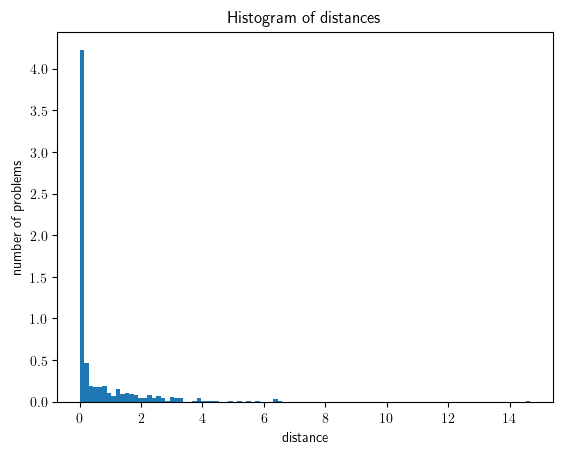
\includegraphics[width=0.48\textwidth]{./Thesis/images/chapter3/example_theta_dist.png}
      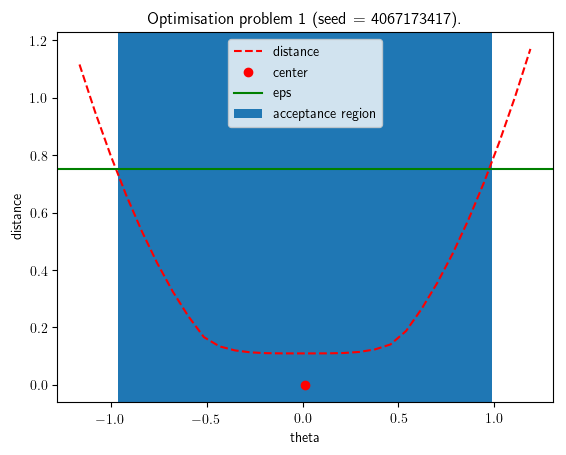
\includegraphics[width=0.48\textwidth]{./Thesis/images/chapter3/example_region.png}
    \end{center}
  \caption{Histogram of distances and visualisation of a specific region.}
  \label{fig:example_training}
\end{figure}
